% ============================================================
\chapter{Barcodes and Persistence Diagrams}
\label{ch:diagrams}
% ============================================================

Persistent homology produces a considerable amount of information: for each dimension, a list of topological features with their birth and death times. How does one visualise and compare these results? Two equivalent representations have established themselves: the \emph{barcode}, where each feature is a horizontal bar whose length measures its persistence, and the \emph{persistence diagram}, where each feature is a point in the upper half-plane. These representations, introduced by Edelsbrunner, Letscher, and Zomorodian in the early 2000s, have become the standard interface between topological theory and applications.

\begin{intuition}
The persistence diagram and the barcode are two equivalent
representations of the result of persistent homology. Each point
$(b, d)$ in the diagram represents a topological feature born at $b$
and dying at $d$. The farther a point is from the diagonal, the more
persistent --- and thus more significant --- the feature.
\end{intuition}

% ============================================================
\section{Persistence Diagrams}
% ============================================================

\begin{definition}[Persistence Diagram]
Let $\{(b_k, d_k)\}_{k=1}^N$ be the set of birth-death pairs from
persistent homology in dimension $p$. The \emph{persistence diagram}
is the multiset:
\[
  \mathrm{Dgm}_p = \{(b_k, d_k) \in \R^2 : b_k < d_k\}
  \cup \Delta
\]
where $\Delta = \{(x, x) : x \in \R\}$ is the diagonal, equipped
with infinite multiplicity.
\end{definition}

\begin{remark}
Adding the diagonal with infinite multiplicity is essential for
correctly defining distances between diagrams
(Chapter~\ref{ch:distances}).
\end{remark}

\begin{center}
\begin{tikzpicture}[scale=1.5]
  % Axes
  \draw[->] (-0.2,0) -- (3.5,0) node[right] {birth $b$};
  \draw[->] (0,-0.2) -- (0,3.5) node[above] {death $d$};
  % Diagonal
  \draw[gray, dashed] (0,0) -- (3.2,3.2);
  % Points
  \fill[blue] (0.2, 2.8) circle (2pt) node[right, font=\small] {$(b_1, d_1)$};
  \fill[blue] (0.5, 1.2) circle (2pt);
  \fill[blue] (0.8, 1.0) circle (2pt);
  \fill[red] (0.3, 0.5) circle (2pt);
  \fill[red] (1.0, 1.2) circle (2pt);
  \fill[red] (1.5, 1.8) circle (2pt);
  % Legend
  \fill[blue] (2.5, 3.2) circle (2pt);
  \node[right, font=\small] at (2.6, 3.2) {$H_0$};
  \fill[red] (2.5, 2.9) circle (2pt);
  \node[right, font=\small] at (2.6, 2.9) {$H_1$};
  % Persistence annotation
  \draw[<->, thin, blue] (0.2, 2.6) -- (0.2, 0.4);
  \node[left, font=\tiny, blue] at (0.15, 1.5) {persistence};
\end{tikzpicture}
\end{center}

\begin{definition}[Persistence]
The \emph{persistence} of a point $(b, d)$ is
$\mathrm{pers}(b,d) = d - b$. The \emph{total persistence} is:
\[
  \mathrm{Pers}_q(\mathrm{Dgm}) = \left(\sum_{(b,d) \in \mathrm{Dgm}}
  (d - b)^q \right)^{1/q}.
\]
\end{definition}

% ============================================================
\section{Barcodes}
% ============================================================

\begin{definition}[Barcode]
The \emph{barcode} is the equivalent representation where each pair
$(b_k, d_k)$ is drawn as a horizontal segment $[b_k, d_k)$. The
segments are stacked vertically.
\end{definition}

\begin{center}
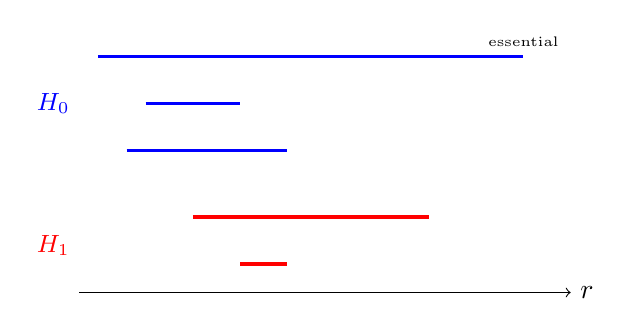
\begin{tikzpicture}[scale=1.2]
  \draw[->] (-0.2,0) -- (5,0) node[right] {$r$};
  % H_0 bars
  \draw[blue, very thick] (0, 2.5) -- (4.5, 2.5);
  \draw[blue, very thick] (0.5, 2.0) -- (1.5, 2.0);
  \draw[blue, very thick] (0.3, 1.5) -- (2.0, 1.5);
  % H_1 bars
  \draw[red, very thick] (1.0, 0.8) -- (3.5, 0.8);
  \draw[red, very thick] (1.5, 0.3) -- (2.0, 0.3);
  % Labels
  \node[left, font=\small, blue] at (-0.2, 2.0) {$H_0$};
  \node[left, font=\small, red] at (-0.2, 0.5) {$H_1$};
  \node[above, font=\tiny] at (4.5, 2.5) {essential};
\end{tikzpicture}
\end{center}

\begin{remark}
The barcode and the persistence diagram contain exactly the same
information. The barcode is often more intuitive for visualization;
the diagram is better suited for mathematical analysis (distances,
stability).
\end{remark}

% ============================================================
\section{Betti Functions}
% ============================================================

\begin{definition}[Betti Function]
The \emph{Betti function} $\beta_p : \R \to \N$ assigns to each
$r \in \R$ the Betti number of the filtered complex at level $r$:
\[
  \beta_p(r) = \dim H_p(K_r).
\]
It is a step function, piecewise non-decreasing.
\end{definition}

\begin{proposition}
The Betti function $\beta_p(r)$ can be read directly from the barcode:
$\beta_p(r)$ is the number of bars containing $r$ in dimension $p$.
\end{proposition}

% ============================================================
\section{Persistence Landscapes}
% ============================================================

\begin{definition}[Persistence Landscape]
Let $\mathrm{Dgm}_p = \{(b_i, d_i)\}$. For each point, define the
tent function:
\[
  \Lambda_i(t) = \max\left(0,\, \min(t - b_i,\, d_i - t)\right).
\]
The \emph{$k$-th persistence landscape} is:
\[
  \lambda_k(t) = k\text{-th largest value of }
  \{\Lambda_i(t)\}_{i=1}^N.
\]
\end{definition}

\begin{keyformulas}[title=\textbf{Persistence Landscape}]
\[
  \lambda_k : \R \to \R_{\geq 0}, \quad
  \lambda_k(t) = \mathrm{kmax}\big\{\Lambda_i(t) : (b_i, d_i)
  \in \mathrm{Dgm}_p\big\}
\]
where $\mathrm{kmax}$ denotes the $k$-th maximum.
\end{keyformulas}

\begin{theorem}[Bubenik, 2015]
Persistence landscapes are elements of a separable Banach space. They
satisfy a strong law of large numbers and a central limit theorem.
\end{theorem}

% ============================================================
\section{Persistence Images}
% ============================================================

\begin{definition}[Persistence Image]
The \emph{persistence image} is obtained by:
\begin{enumerate}
  \item Transforming each point $(b, d)$ to $(b, d-b)$
        (birth-persistence coordinates).
  \item Placing a Gaussian $\mathcal{N}((b_i, p_i), \sigma^2 I)$
        centered at each transformed point.
  \item Weighting by a weight function $w(b, p)$ (typically increasing
        in $p$).
  \item Discretizing on a grid to obtain a matrix.
\end{enumerate}
\end{definition}

\begin{keyformulas}[title=\textbf{Persistence Image}]
\[
  \rho(x, y) = \sum_{i=1}^{N} w(b_i, p_i) \cdot
  \frac{1}{2\pi\sigma^2}
  \exp\left(-\frac{(x - b_i)^2 + (y - p_i)^2}{2\sigma^2}\right)
\]
where $p_i = d_i - b_i$ is the persistence of the $i$-th point.
\end{keyformulas}

% ============================================================
\section{Implementations}
% ============================================================

\begin{codeblock}[title=\textbf{Visualizing Diagrams and Barcodes}]
\begin{minted}{python}
import numpy as np
from ripser import ripser
from persim import plot_diagrams
import matplotlib.pyplot as plt

# Noisy circle
theta = np.linspace(0, 2*np.pi, 100, endpoint=False)
X = np.column_stack([np.cos(theta), np.sin(theta)])
X += 0.1 * np.random.randn(*X.shape)

result = ripser(X, maxdim=1)
dgms = result['dgms']

fig, axes = plt.subplots(1, 3, figsize=(15, 4))

# Persistence diagram
plot_diagrams(dgms, ax=axes[0])
axes[0].set_title("Persistence Diagram")

# Barcode
for dim, dgm in enumerate(dgms):
    color = ['blue', 'red'][dim]
    offset = 0 if dim == 0 else len(dgms[0])
    for k, (b, d) in enumerate(dgm):
        if np.isinf(d):
            d = max(dgm[np.isfinite(dgm[:, 1]), 1].max(), b + 0.5)
        axes[1].plot([b, d], [k + offset, k + offset],
                     color=color, linewidth=2)
axes[1].set_title("Barcode")
axes[1].set_xlabel("$r$")

# Persistence landscape
t = np.linspace(0, 2.5, 500)
dgm1 = dgms[1]
dgm1_finite = dgm1[np.isfinite(dgm1[:, 1])]
tents = np.array([np.maximum(0, np.minimum(t - b, d - t))
                   for b, d in dgm1_finite])
if len(tents) > 0:
    landscape_1 = np.sort(tents, axis=0)[::-1]
    for k in range(min(3, len(landscape_1))):
        axes[2].plot(t, landscape_1[k], label=f"$\\lambda_{k+1}$")
    axes[2].legend()
axes[2].set_title("Persistence Landscapes ($H_1$)")

plt.tight_layout()
plt.savefig("persistence_representations.pdf")
\end{minted}
\end{codeblock}

\begin{codeblock}[title=\textbf{Persistence Images with giotto-tda}]
\begin{minted}{python}
from gtda.homology import VietorisRipsPersistence
from gtda.diagrams import PersistenceImage
import numpy as np

# Data
theta = np.linspace(0, 2*np.pi, 100, endpoint=False)
X = np.column_stack([np.cos(theta), np.sin(theta)])
X += 0.1 * np.random.randn(*X.shape)

# giotto-tda pipeline
VR = VietorisRipsPersistence(homology_dimensions=[0, 1])
diagrams = VR.fit_transform(X[np.newaxis, :, :])

PI = PersistenceImage(sigma=0.1, n_bins=20)
images = PI.fit_transform(diagrams)
print(f"Persistence image shape: {images.shape}")
\end{minted}
\end{codeblock}

% ============================================================
\section{Persistence Entropy}
% ============================================================

\begin{definition}[Persistence Entropy]
Let $\mathrm{Dgm} = \{(b_i, d_i)\}_{i=1}^N$ be a persistence diagram
(finite points only). The \emph{persistence entropy} is:
\[
  E(\mathrm{Dgm}) = -\sum_{i=1}^{N} p_i \log p_i, \quad
  p_i = \frac{d_i - b_i}{\sum_{j=1}^N (d_j - b_j)}.
\]
It measures the complexity of the distribution of lifetimes.
\end{definition}

% ============================================================
\section{Betti Curve}
% ============================================================

\begin{definition}[Betti Curve]
The \emph{Betti curve} is the function $\beta_p : \R \to \N$ defined by:
\[
  \beta_p(t) = \abs{\{(b_i, d_i) \in \mathrm{Dgm}_p : b_i \leq t < d_i\}}.
\]
\end{definition}

This curve is directly related to the barcode: it counts the number of
active bars at each time $t$.

% ============================================================
\section{Persistence Silhouettes}
% ============================================================

\begin{definition}[Persistence Silhouette]
The \emph{persistence silhouette} of order $q > 0$ is the weighted
average of tent functions:
\[
  \phi_q(t) = \frac{\sum_i (d_i - b_i)^q \cdot \Lambda_i(t)}
  {\sum_i (d_i - b_i)^q}.
\]
For $q = 1$, this is the arithmetic mean weighted by persistence.
\end{definition}

% ============================================================
\section{Statistics on Diagrams}
% ============================================================

\begin{theorem}[Fr\'echet Mean]
Let $\mathcal{D} = \{D_1, \ldots, D_n\}$ be a sample of persistence
diagrams. The \emph{Fr\'echet mean} is:
\[
  \bar{D} = \arg\min_{D} \sum_{i=1}^n W_2(D, D_i)^2
\]
where $W_2$ is the $2$-Wasserstein distance. This minimum exists but
is not necessarily unique.
\end{theorem}

\begin{proposition}
Persistence landscapes, being elements of a Banach space, admit a
well-defined mean:
\[
  \bar{\lambda}_k(t) = \frac{1}{n} \sum_{i=1}^n \lambda_k^{(i)}(t).
\]
\end{proposition}

% ============================================================
\section{Exercises}
% ============================================================

\begin{exercise}
Construct the persistence diagram and barcode for a Vietoris--Rips
filtration of $6$ points equally spaced on a circle.
\end{exercise}

\begin{exercise}
Implement in Python the computation of a persistence landscape from a
persistence diagram. Test on a noisy circle.
\end{exercise}

\begin{exercise}
Compute the persistence image of a cloud of $200$ points on a torus.
Vary the parameter $\sigma$ and observe the effect on the image.
\end{exercise}

\begin{exercise}
Show that persistence entropy is maximal when all lifetimes are equal,
and minimal (zero) when only one pair has nonzero persistence.
\end{exercise}

\begin{exercise}
Compare the persistence landscapes of a circle, a torus, and a sphere
sampled with noise. What differences do you observe?
\end{exercise}
